\chapter{Electrostatically loaded 3D elastic beam}

\modinfo{Solvers}{\Idx{StressSolve}, Idx{StatElecSolve}}
\modinfo{Tools}{\Idx{ElmerGrid}, editor}
\modinfo{Dimensions}{3D, Steady-state}

\section{Case definition}


\section{Results}

\begin{figure}[h]
  \centerline{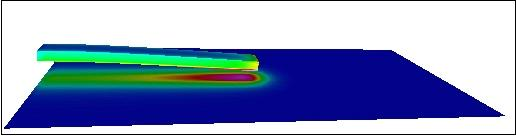
\includegraphics[width=0.8\textwidth]{electric_force}}
  \caption{An elastic beam bended by the electrostatic force due to a
          potential difference between the beam and the bottom
          plate. The electric potential is calculated in the volume
          surrounding the beam although the solution or the mesh are
          not shown.}
\end{figure}
